\pagebreak
\section{Capacitors}
\hrule
\vspace{.5cm}
\textbf{What happens if we pull apart a parallel plate capacitor?}
\begin{list}{-}{}
\item \(Q\) remains constant
\item \(E\) increases
\item \(\Delta V\) increases 
\item \(C\) decreases 
\item \(U\) increases
\end{list}

\subsection{Dielectrics}\label{sec:dielectrics}
\begin{list}{-}{}
\item Material where positive and negative charges in individual molecules can change, but no through the entire material
\item When placed between a capacitor all of the charges align themselves to the field
\item This creates a material full of little dipoles 
\item This induced field is the \textit{opposite} of the one from the plates 
\item This has the effect of \textit{reducing} the electric field within the capacitor, which then reduces the potential diff (\(V\)), which then \textit{increases} the capacitance 
\item \[C = \frac{Q}{V}\]  
\item The amount a capacitance increases is called the \gls{var:dielectricConstant} and is calculated via \(C_{old} = \kappa C_{new}\)
\end{list}

\pagebreak
\begin{example}
    Adding a Dielectric to a Capacitor
    \vspace{.2cm}
    \hrule
    \vspace{.2cm}
    \begin{center}
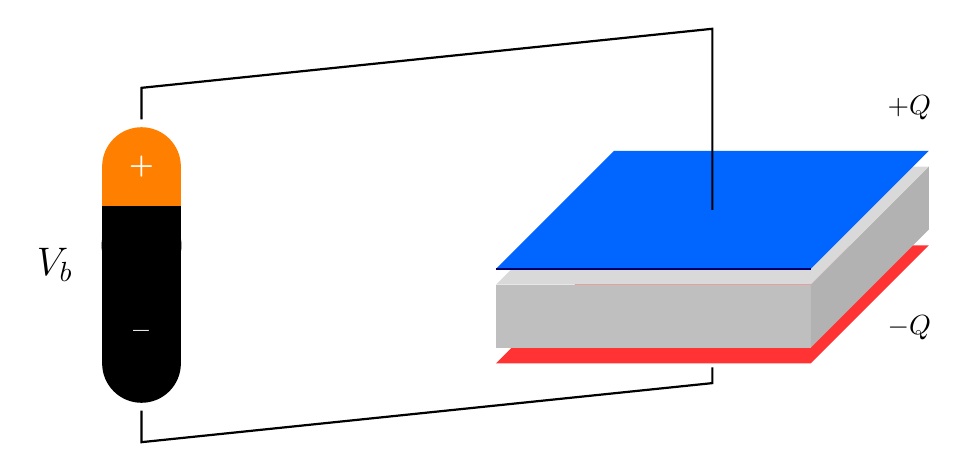
\begin{tikzpicture}[
    x={(1cm,0cm)}, y={(0.5cm,0.5cm)}, z={(0cm,1cm)},
    >=stealth
]


    % --- The Battery (Stylized D-Cell) ---
    % Bottom black section
    \fill[black] (-4.5,0,0) circle (0.5cm);
    \fill[black] (-5,0,0) rectangle (-4,0,2);
    \draw[black, fill=black] (-4.5,0,1.5) circle (0.5cm);
    
    % Top orange section
    \fill[orange] (-5,0,2) rectangle (-4,0,2.5);
    \fill[orange] (-4.5,0,2.5) circle (0.5cm);
    
    
    \node at (-5.6,0,1.25) {\Large $V_b$};
    \node[white] at (-4.5,0,2.5) {\textbf{+}};
    \node[white] at (-4.5,0,0.4) {\textbf{--}};

    % --- Capacitor & Dielectric ---
    % Bottom Plate Edge
    \draw[thick, white] (0,0,0) -- (4,0,0);
    \fill[red!80] (0,0,0) -- (4,0,0) -- (4,3,0) -- (0,3,0) -- cycle;
    
    % Dielectric Volume
    \fill[gray!50] (0,0,.2) -- (4,0,.2) -- (4,0,1) -- (0,0,1) -- cycle; % Front
    \fill[gray!60] (4,0,.2) -- (4,3,.2) -- (4,3,1) -- (4,0,1) -- cycle; % Side
    \fill[gray!30] (0,0,1) -- (4,0,1) -- (4,3,1) -- (0,3,1) -- cycle; % Top
    
    % Dielectric Label
    \node[text=gray] at (2,1.5,0.6) {Dielectric \hspace{0.2cm} \Large $\kappa$};

    % Top Plate
    \fill[blue!60!cyan] (0,0,1.2) -- (4,0,1.2) -- (4,3,1.2) -- (0,3,1.2) -- cycle;
    \draw[thick, blue!40!black] (0,0,1.2) -- (4,0,1.2); 
    
    % Charges
    \node at (4.5, 1.5, 2.5) {$+Q$};
    \node at (4.5, 1.5, -0.3) {$-Q$};

    % --- Wiring ---
    \draw[thick] (-4.5,0,3.1) -- (-4.5,0,3.5) -- (2,1.5,3.5) -- (2,1.5,1.2); 
    \draw[thick] (-4.5,0,-.6) -- (-4.5,0,-1) -- (2,1.5,-1) -- (2,1.5,-.8); 

\end{tikzpicture}

\begin{list}{-}{}
\item Capacitance increases 
\item \(V_c = V_b\)
\item Because \(C = \frac{Q}{V} \rightrightarrows Q\uparrow\) 
\item Because \( U = \frac{1}{2} Q V_c \rightrightarrows U \uparrow\)
\end{list}
\end{center}
\end{example}

\subsection{Capacitors in Parallel}
\begin{list}{-}{}
\item When wired in parallel they can be treated as one capacitor with a larger area
\item this equivalent capacitor has\dots
\[V_{equiv} = V_1 = V_2 \qquad C_{equiv} = C_1 + C_2, \qquad Q_{equiv} = Q_1 + Q_2\]
\end{list}

\subsection{Capacitor in series}
\begin{list}{-}{}
\item When wired in series they act like a capacitor with a large distance 
\item This equivalent capacitor has \dots
\[Q_{equiv} = Q_1 = Q_2 \qquad \frac{1}{C_{equiv}} = \frac{1}{C_1} + \frac{1}{C_2}, \qquad V_{equiv} =V_1 + V_2\]
\end{list}

\pagebreak
\begin{example}
    \begin{center}        
    \textbf{Combination of Capacitors}
    \vspace{.25cm}
    \hrule 
    \vspace{.25cm}


\begin{circuitikz}[american]
    % Main battery loop and C1
    \draw (0,0) to[battery2, l={$V_b=12$\,V}] (0,3)
          to[short] (2,3)
          to[C, l={$C_1=1$\,mF}] (2,0)
          to[short] (0,0);
          
    % Branch for C2 and C3
    \draw (2,3) to[short] (3,3)
          to[C, l={$C_2=2$\,mF}] (5,3)
          to[short] (6,3)
          to[C, l={$C_3=3$\,mF}] (6,0)
          to[short] (2,0);
\end{circuitikz}

\vspace{.5cm}
Simply into single capacitors 
\[C_2, C_3 \rightarrow \frac{1}{C_{23}} = \frac{1}{C_2} + \frac{1}{C_3} = 1.2\text{mF}\]
\[C_1, C_{23} \rightarrow C_1 + C_{23} = C_{123}= 2.2\text{mF}\]

\end{center}

\end{example}